\documentclass[12pt, a4paper]{article} %Definerer skriftstørrelse, arktrype( eks a0paper, ..., a6paper, letterpaper....), dokumenttype(article, report, book, letter, beamer(presentasjon).   
\usepackage[font=small, labelfont=bf]{caption}
\usepackage{graphicx}
\usepackage{pdfpages}
\usepackage{amsmath, amssymb} %  matematiske funskjoner og symboler. 
\usepackage{listings}
\usepackage{url} % urls in the bibliograpy
\usepackage[utf8]{inputenc} % 
\usepackage{float}  %
\usepackage{subcaption} % NOT compatible with the subfig package
\usepackage{authblk}
\usepackage{siunitx}
\usepackage[parfill]{parskip}


\usepackage[  
left=20mm,
 right=20mm,
 top=10mm,
 bottom=20mm]{geometry} % kan endre på marger 
%%%%%%%%%%%%%%%%%%%%%%%%%%%%%%%%%%%%%%%%%%%%%%%%%%%%%%%%%%%%%%%%
% Gode infosider:
% https://no.sharelatex.com/learn/Creating_a_document_in_LaTeX 
% https://no.sharelatex.com/learn/Page_size_and_margins
 
%%%%%%%%%%%%%%%%%%%%%%%%%%%%%%%%%%%%%%%%%%%%%%%%%%%%%%%%%%%%%%%%
% Det som inkluderes i \maketitle
\title{Øving 2\\ TDT4200}
\author[1]{Anette Fossum Morken}
\date{}
%%%%%%%%%%%%%%%%%%%%%%%%%%%%%%%%%%%%%%%%%%%%%%%%%%%%%%%%%%%%%%%
\begin{document}
\maketitle

\section*{Del 1, oppgave 1}
\subsection*{a}
skrives om lockblock?? pipeline minnehierarki hetero/homo? numa/cluster?
\subsubsection*{i)}
Nivida Maxwell Nvidia Maxwell har homogene kjerner med tråder og er NUMA .
\subsubsection*{ii)}
ARM big.LITTLE er en samling av to forskjelige prosessorer. Den ene prosessoren er energikrevende og den andre er lite energikrevende slik at når enkle oppgaver, som tekstbehandling, skal gjøres gjøres det på den mindre energikrevende prosessoren og når tyngre oppgaver skal gjøres gjøres de på den mer energikrevende prosessoren. Siden den tydelig består av to forskjellige prosessorer har denne heterogenious kjerner 

\subsubsection*{iii)}
vilje@NTNU er en superdatamaskin som består av prosessorere i kluster. Hver prosessor igjen bastår av et vist antall tråder. Prosessorene og trådene er organisert slik at tingangen til alle trådene ikke er lik og dermed er vilje NUMA.
\subsubsection*{iv)}
En vanlig CPU i dag består av flere like kjerner hvor hver kjerne består av et vist antall tråder som kan brukes samtidig.  
\subsection*{b}
SIMT passer inn i Flynns taksonomi i SIMD, der det på Nivida er en instruksjon flere tråder vil det i Flynns taksonomi bli en instruksjon multiple data. 

\subsection*{c}
\subsubsection*{i)}
Nivida Maxwell passer inn i Flynns både som SIMD og MIMD siden den har mulighet til å gjøre plere ting på en gang.
\subsubsection*{ii)}
ARM big.LITTLE blir i dag mest sett på som SIMD, men siden den består av to forkjellige prosessorere kan den i teorien gjøre to forskjellige oppgaver samtidig.
\subsubsection*{iii)}
vilje@NTNU MIMD
\subsubsection*{iv)}
En vanlig CPU SIMD


\section*{Del 1, oppgave 2}
\subsection*{a}
Tråder er organisert i blokker, bokker er organisert i gridd. Blokkene er helt uangengige av hverandre og kan ikke kommunisere, mens trådene i en blokk kan komunisere med hverandre. 

\section*{b}
Setter opp ligninger for tiden GPUen vil bruke og CPUen vil bruke:
\begin{align}
GPU=\frac{2n}{r}+\frac{5n}{r}+5h_{GPU}n7h_{GPU}log_2(n) \nonumber \\
CPU=5h_{CPU}n7h_{CPU}log_2(n)
\label{alg}
\end{align}
der $h_{GPU}=1$, $h_{CPU}=10$, $r$ er båndbredden og $n$ er mengde data som overføres. Det lønner seg å bruke GPUen når $GPU>CPU$ det finnes ved å regne ut $GPU$ og $CPU$ for mange forskjellige $n$ og plotte dem og se hvor de krysser hverandre slik at $GPU>CPU$.
 Med den oppgitte algoritmen vil det ta kortest til å kjøre på GPUen hvis $n \geqslant 1$, dette kan sees ved å studere plottet i figur \ref{GPU-CPU}. For de fleste andre programmer er ikke dette riktig. Vanligvis vil det være raskest å kjøre programmer der $n$ er liten på CPUen siden minneoverføringen til og fra GPUen er tidkrevende. 
\begin{figure}
\centering
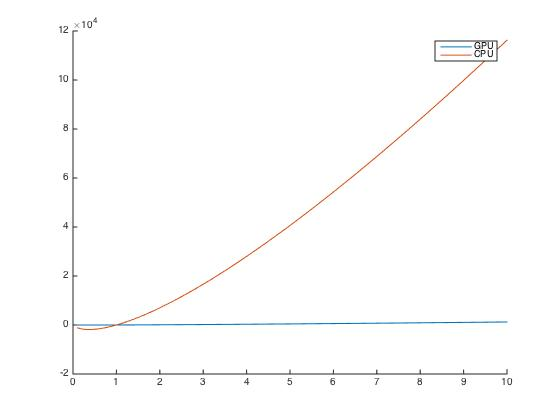
\includegraphics[width=0.5\textwidth]{GPU-CPU.jpg} 
\caption{Plottet viser kjøretiden for et program gitt med kjøretidene i \eqref{alg}}
\label{GPU-CPU}
\end{figure}

\subsection*{c}
Kernel2 vil være raskest siden her blir alle trådene satt i arbeid. I kernel1 looper man gjennom trådene og gir bare et utvalg av trådene arbeid. Hvis trådene i en warp har fått forskjellige instruksjoner vil de bli kjørt serielt og siden alle trådene ikke har samme instruksjon i kernel1 vil denne kjøres serielt. I kernel2 får alle trådene i hver blokk samme instruksjon og vil derfor kjøres parallelt.

\subsection*{d}
\subsubsection*{i)}
Warps er samlinger med tråder. Hvis trådene utfører samme operasjon kan de kjøres paralellt, men har de forskjellige oppgaver må de kjøres serielt.
\subsubsection*{ii)}
Occupancy gir hvor stor andel av tilgjengelige warps som er i bruk. Man kan se også se på det som hvor mange av trådene som står og venter på å få arbeid. 
\subsubsection*{iii)}
Minne fortetting(coalescing) er å slå sammen flere minneoverføringer mellom minet og tråder til en overføring. Det gjør at et gitt antall tråder i en warp kan hente ut informasjon fra minnet på en gang og tiden det tart for alle å hente ut informasjonen er samme som en trå hadde brukt om man ikke benyttet seg av coalescing. På denne måten kan man redusere kjøretiden til programmet.
\subsubsection*{iv)}
Lokalt minne er minne som en tråd kun har tilgang til skal en tråd ha informasjon fra en annen må dette deles gjennom message passing.
\subsubsection*{v)}
Delt minne er at alle trådene i en blokk har tilgang til informasjonen som ligger her.

\section*{Del 2, oppgave 1}
\subsection*{c}
TIden ble tatt på forskjellige steder i koden, hele programmet, minneoverforingen fra CPUen til GPUen og for minneoverføringen CPU-GPU og tilbake og invertringen av bildet. Hele programmet bruker rundt $0,19\cdot 10^9$ns, minneoverføringen CPU-GPU og tilbake og invertringen av bildet bruker rundt $0,63\cdot 10^6$ns og minneoverføringen bruker $0,23 \cdot 10^6$ns

antall prosent tiden brukt til minneoverføringen er av hele kjøretiden: 
antall prosent tiden brukt til minneoverføringen er av selve oppaven til programmet:

DEt første man kan merke seg at I/O tar mye tid, så monneoverføringen er ikke den største tidstyven i dette programmet, men når man ser på CPU-GPU og tilbake og invertringen av bildet ser man at minneoverføring er en prosess som tar tid.





\end{document}
